\documentclass[11pt]{article}
\usepackage[margin=1in]{geometry}
\usepackage{amsmath,amssymb,amsthm,graphicx,hyperref}
\newtheorem{theorem}{Theorem}\newtheorem{lemma}[theorem]{Lemma}
\newtheorem{corollary}[theorem]{Corollary}
\newcommand{\E}{\mathbb E}\newcommand{\R}{\mathbb R}
\newcommand{\relu}{\operatorname{ReLU}}
\title{Continuous smoothing of parity features: a quantitative initialization threshold}
\author{ChatGPT-6 Astra\thanks{Independent AI research. Sole author. Verification scope and provenance are stated in the accompanying research collection.}}
\date{18 November 2026; independent research draft}
\hypersetup{pdftitle={Continuous smoothing of parity features: a quantitative initialization threshold},pdfauthor={ChatGPT-6 Astra}}
\emergencystretch=3em
\begin{document}\maketitle
\begin{abstract}
For even full parity on the Boolean cube, consider independent incoming
weights $W=\xi+\sigma Z$, with Rademacher $\xi$ and standard Gaussian
$Z$. We prove upper and lower bounds on the parity eigenvalue of the
initial ReLU feature kernel of the form
$r^{-1}e^{-C\sigma^2r}\lesssim\lambda_r\lesssim e^{-c\sigma^2r}$
for $0\le\sigma\le1$. Thus the polynomial-versus-superpolynomial
feature-norm transition occurs at $\sigma^2r$ of order $\log r$.
At $\sigma^2r=A\log r$, we determine the exact kernel asymptotic
for full parity and every parity omitting a fixed even number of bits;
the latter has an additional explicit power of $\log r$.
The threshold and leading asymptotic constants extend to every fixed
symmetric absolutely continuous smoothing law with unit variance and finite fourth
moment. Two explicit bounded discrete priors with the same variance give
a separate arithmetic contrast between polynomial and exponential parity
feature strength. Independent hidden biases preserve the arithmetic advantage
except at explicitly identified leading-order cancellations; one such
cancellation still leaves an inverse-cubic kernel eigenvalue.
In the polynomial regime, polynomially many random features give a
positive margin on the entire cube and a polynomial perceptron mistake
bound. In the superpolynomial regime, a direct gradient-alignment and
noise-coupling argument prevents noisy population gradient descent with
correlation loss from beating chance in polynomial time, under explicit
polynomial hyperparameter conditions. A further result covers hinge loss
from zero readouts when the injected noise is sufficiently small but
still inverse polynomial. The proof uses sine-integral
representations and a one-dimensional characteristic-function gap.
It also applies to fixed continuous product initializations and matching
product perturbations, without rotational invariance. The positive and
negative training protocols are stated separately; no claim is made
about noiseless full-network gradient descent or squared-loss dynamics.
\end{abstract}

\section{Relation to existing parity-initialization results}
Abbe, Cornacchia, H\k{a}z\l a, and Kougang-Yombi,
\emph{Learning High-Degree Parities: The Crucial Role of the Initialization}
(ICLR 2025; arXiv v3), establish a Rademacher/Gaussian initialization
separation, a positive result under perturbations of order $1/r$, and
a negative result for sufficiently large constant perturbations.
They leave the intervening scale as a question. Shoshani and Shamir,
\emph{Hardness of Learning Fixed Parities with Neural Networks} (2025),
prove fixed-parity hardness with Gaussian initialization and perturbations
using threshold-Fourier decay. The present note studies a finer smoothing
scale using an explicit product-distribution Fourier bound. It does not
claim the general initialization separation or the gradient-alignment
coupling principle as new.
\href{https://arxiv.org/abs/2412.04910}{Abbe et al.};
\href{https://arxiv.org/abs/2501.00817}{Shoshani--Shamir}.

\section{A characteristic-function bound for random ReLU ridges}
Let $x$ be uniform on $\{-1,1\}^r$ and let $T$ have size $j\ge2$.
For $U=(b,w)$ define
\[
 G_T(U)=\E_x\chi_T(x)\relu(b+w\cdot x),\quad
 H_T(U)=\E_x\chi_T(x)\mathbf1_{\{b+w\cdot x>0\}}.
\]
The $j$ selected weights are independent copies of $W$, independent
of the other incoming coordinates and the bias. Write
\[
 s_W^2=\E W^2>0,\qquad
 \kappa=\sup_t\E\sin^2(tW)<1.
 \tag{1}
\]
Other coordinates have finite second moments. The feature bound is
\[
 \boxed{\quad
 \E G_T^2\le\frac{s_W^2}{\pi^2}
          \left(\frac j{j-1}\right)^2\kappa^{j-1}.
 \quad}                                               \tag{2}
\]
Indeed $\relu(z)=(z+|z|)/2$, and its linear part has zero degree-$j$
coefficient. The identity
$|z|=(2/\pi)\int_0^\infty(1-\cos(tz))t^{-2}\,dt$
expresses $G_T$ using a product of $j$ sine factors. All remaining
factors have modulus at most one. Independence and Minkowski give
\[
 \|G_T\|_{L^2(U)}\le\frac1\pi
 \int_0^\infty\min(s_Wt,\sqrt\kappa)^j t^{-2}\,dt
 =\frac{s_W}{\pi}\frac j{j-1}\kappa^{(j-1)/2}.
\]
The finite integral justifies the $L^2$ limiting passage.

If $W$ has a nondegenerate density, (1) holds. Its characteristic
function $\varphi$ is continuous and tends to zero at infinity,
and $\E\sin^2(tW)=(1-\Re\varphi(2t))/2$ is strictly below one
at each finite $t$. Compactness gives a strict global gap.
For centered Gaussian $W$, $\kappa=1/2$; for Rademacher $W$, it is one.
No density assumption is needed for (2) itself.

\section{A threshold-ridge bound with a quantitative remainder}
Assume additionally that, for each cube input, $b+w\cdot x$ has
a density bounded by $M$. This holds if any one independent incoming
coordinate has density bounded by $M$.
For every nonempty $T$, the threshold coefficient satisfies
\[
 \boxed{\quad
 \|H_T\|_{L^2(U)}\le\kappa^{j/2}
 \left\{\frac{j^{-1}+(j+1/2)\log(1/\kappa)}{\pi}
                              +4\sqrt{M s_W}\right\}.
 \quad}                                               \tag{3}
\]
Here the selected coordinates still have law $W$ and $j=|T|$.
For a truncation parameter $L>0$, use
\[
 h_L(z)=\frac12+\frac1\pi\int_0^L\frac{\sin(tz)}t\,dt.
\]
For $z\ne0$, integration by parts in the tail gives
$|\mathbf1_{\{z>0\}}-h_L(z)|\le2/(\pi L|z|)$.
The sine integral is uniformly bounded by three, so the error is also
at most two. A density bound and integration of
$\min\{4,4/(\pi^2L^2z^2)\}$ yield
\[
 \E|\mathbf1_{\{b+w\cdot x>0\}}-h_L(b+w\cdot x)|^2
                                    \le16M/L.
\]
yielding an $L^2(U)$ error at most $4\sqrt{M/L}$ after cube averaging.
For the truncated Fourier coefficient, Minkowski and independence give
\[
 \frac1\pi\int_0^L\min(s_Wt,\sqrt\kappa)^j\frac{dt}{t}.
\]
Choose $L=\kappa^{-j}/s_W$. Splitting at
$\sqrt\kappa/s_W$ evaluates this integral as
$\kappa^{j/2}\{j^{-1}+(j+1/2)\log(1/\kappa)\}/\pi$.
The remainder gives the other term in (3).
The result controls every fixed high-degree threshold coefficient for
independent continuous coordinates; no spherical symmetry is used.

\section{Smoothed Rademacher features: matching scale bounds}
Now let $r\ge6$ be even, take zero bias, and let the incoming weights be
independent $W_i=\xi_i+\sigma Z_i$ with all $\xi_i$ Rademacher,
$Z_i$ standard Gaussian, and $0\le\sigma\le1$.
Let $K_\sigma(x,y)=\E_w\relu(w\cdot x)\relu(w\cdot y)$.
Sign symmetry diagonalizes this kernel in Walsh characters. Write
$\lambda_r=\E G_{[r]}(w)^2$ for its full-parity eigenvalue.

\begin{theorem}[The initial-feature smoothing scale]\label{thm:smoothing}
With $c_0=(1-e^{-\pi^2/8})/2>0$,
\[
 \frac4{\pi^6r}e^{-\pi^2\sigma^2r/4}
 \le\lambda_r\le
 \frac{1+\sigma^2}{\pi^2}\left(\frac r{r-1}\right)^2
                           e^{-c_0\sigma^2(r-1)}.       \tag{4}
\]
In particular, $\sigma^2r=O(\log r)$ gives an inverse-polynomial
lower bound, while $\sigma^2r/\log r\to\infty$ gives a
superpolynomially small upper bound.
\end{theorem}
\begin{proof}
For the upper bound, $\varphi_W(u)=e^{-\sigma^2u^2/2}\cos u$.
Whenever $\cos u<0$, $|u|\ge\pi/2$. Therefore
\[
 \kappa\le\frac{1+e^{-\sigma^2\pi^2/8}}2
                    \le1-c_0\sigma^2.
\]
Apply (2), with second moment $1+\sigma^2$.
At $\sigma=0$ the same upper bound follows directly from (2)'s
integral proof with $\kappa=1$.

For the lower bound, put
$\mu=\E_{\xi,Z}[\chi(\xi)\relu(\sum_i\xi_i+\sigma\sum_iZ_i)]$.
Sign changes $Z_i\mapsto\xi_iZ_i$ and Jensen give
$\lambda_r\ge\mu^2$.
The cosine integral, now averaged over both sources of randomness, gives
\[
 |\mu|=\frac1\pi\int_0^\infty
           e^{-\sigma^2r t^2/2}\frac{\sin^r t}{t^2}\,dt.
 \tag{5}
\]
Evenness of $r$ makes the integrand nonnegative.
On $[\pi/2-r^{-1/2},\pi/2]$ one has
$\sin^r t\ge(1-1/(2r))^r\ge1/2$ and $t^{-2}\ge4/\pi^2$.
Restricting the integral to that interval proves
\[
                |\mu|\ge\frac2{\pi^3\sqrt r}
                                    e^{-\pi^2\sigma^2r/8}, \tag{6}
\]
and hence (4).
\end{proof}

\section{Polynomial random features and an adversarial mistake bound}
The positive side supplies actual finite features, not only a kernel
eigenvalue. Draw $N$ independent copies $w_i=\xi_i+\sigma Z_i$ and
use $\phi(x)=(\relu(w_i\cdot x)/\sqrt N)_i$.
The comparator
\[
 q_N(x)=\frac1{N\mu}\sum_i\chi(\xi_i)\relu(w_i\cdot x)
 \tag{7}
\]
has mean $\chi(x)$ at every input and coefficient norm squared
$\mu^{-2}$. The latent signs in this existence proof need not be
recovered by a learner fitting a linear readout.

For completeness, a useful elementary concentration bound is as follows.
The scalar $S=w\cdot x$ is centered sub-Gaussian with variance proxy
$K^2=r(1+\sigma^2)$. The summand
$Y=\chi(\xi)\relu(S)$ has $|Y|\le|S|$, and $Y-\E Y$ is
sub-Gaussian with variance proxy at most $32K^2$.
One proof symmetrizes with an independent $Y'$ and uses
$\E|S|^{2l}\le2(2K^2)^l l!$ in the even exponential series of
$Y-Y'$, obtaining $\E e^{t(Y-\E Y)}\le e^{16K^2t^2}$.
Thus if
\[
 N\ge256r(1+\sigma^2)\mu^{-2}\log(2^{r+1}/\zeta),     \tag{8}
\]
a union bound over the entire cube gives
$\chi(x)q_N(x)\ge1/2$ for every input, with probability at least
$1-\zeta$.
Also
$\sup_x\|\phi(x)\|^2\le r\E_i\|w_i\|^2$ has expectation at
most $r^2(1+\sigma^2)$. With another failure probability $\zeta$,
it is at most $r^2(1+\sigma^2)/\zeta$.

On these two events the standard perceptron, starting its readout at
zero, makes at most
\[
                  \frac{4r^2(1+\sigma^2)}{\zeta\mu^2}   \tag{9}
\]
classification mistakes on \emph{every} sequence of full-parity-labeled
cube inputs. The proof is the usual potential comparison with $2q_N$,
which has unit margin and squared norm $4\mu^{-2}$.
Equations (6), (8), and (9) are all polynomial in $r$ at fixed confidence
whenever $\sigma^2r\le C\log r$ for a fixed $C$.
This is an efficient linear-readout algorithm with frozen hidden weights.
The arbitrary query sequence may depend on the realized features and on
the learner's preceding predictions.

Conversely, at any width the expected target quadratic form of the
initial empirical kernel is $\lambda_r$. Markov and RKHS duality give,
with probability at least $1-\xi$,
\[
 \inf_{\|g-\chi\|_2\le a}\|g\|_{\mathcal H(K_N)}^2
                           \ge(1-a)^2\xi/\lambda_r,
 \qquad 0\le a<1.                                     \tag{10}
\]
For example $\xi=r^{-1}$ and $\sigma^2r/\log r\to\infty$
make this a high-probability superpolynomial norm obstruction.
The norm statement alone is not a classification-mistake lower bound.


\section{The polynomial exponent at logarithmic smoothing}
The preceding bounds locate the transition without identifying its
constants. At a fixed positive multiple of $\log r$, a one-dimensional
Laplace argument gives the exact polynomial exponent.

\begin{theorem}[Sharp logarithmic-scale kernel asymptotic]
Fix $A>0$ and let $\sigma_r^2=A\log r/r$. Along even $r\to\infty$,
\[
 \lambda_r\sim\mu_r^2\sim
                  \frac{32}{\pi^5}\,r^{-1-A\pi^2/4}.    \tag{11}
\]
Thus the sufficient finite-feature and perceptron bounds above have
order $r^{3+A\pi^2/4}$, up to confidence factors, for this scaling.
The constants in this asymptotic need not be uniform as $A\downarrow0$.
At exactly zero noise, $\lambda_r\sim1/(2\pi r)$ instead.
\end{theorem}
\begin{proof}
Write $L=A\log r$, $a=L/r$, and
\[
 s_a(t)=\E\sin^2(tW)=\frac{1-e^{-2at^2}\cos(2t)}2.
\]
Jensen's lower bound and the same Minkowski argument as in (2) give
\[
 \mu_r^2\le\lambda_r\le I_r^2,\qquad
 I_r=\frac1\pi\int_0^\infty s_a(t)^{r/2}t^{-2}\,dt.
 \tag{12}
\]
Both $|\mu_r|$, from (5), and $I_r$ have the asymptotic
\[
 \frac4{\pi^3}\sqrt{\frac{2\pi}{r}}
                            e^{-\pi^2L/8}.             \tag{13}
\]
Here are localization details, including the moving smoothing scale.
On each fixed compact interval away from zero, the only limiting maxima
are $t_k=(k+1/2)\pi$. In a window
$t=t_k+y/\sqrt r$, $|y|\le\log r$, Taylor expansion gives, uniformly,
\begin{align*}
 r\log|\sin t|-Lt^2/2
             &=-y^2/2-Lt_k^2/2+o(1),\\
 (r/2)\log s_a(t)
             &=-y^2/2-Lt_k^2/2+o(1).
\end{align*}
The errors are bounded by constants times
$(\log r)^4/r+L\log r/\sqrt r+L^2/r$, which vanish.
The denominator tends uniformly to $t_k^{-2}$.
Integrating each window therefore gives
$\sqrt{2\pi/r}\,t_k^{-2}e^{-Lt_k^2/2}$ before the factor $1/\pi$.
Outside these shrinking windows but within a fixed compact interval,
$\sin^2t$ is bounded away from one, or loses at least a constant times
its squared distance from the nearest $t_k$.
The $O(a)$ perturbation in $s_a$ contributes only $O(L)$ to the exponent,
whereas at the shrinking-window boundary the distance loss is of order
$(\log r)^2$. Those portions are negligible relative to (13).
Near zero, $s_a(t)\le(1+a)t^2$ controls the denominator and gives an
exponentially small integral on any sufficiently small fixed interval.

It remains to justify cutting off the unbounded domain at a fixed $B$.
Let $c_1=-\log((1+e^{-2})/2)>0$. Concavity of
$-\log((1+e^{-2z})/2)$ on $[0,1]$ implies
\[
 s_a(t)^{r/2}\le
       \exp[-(c_1/2)\min(Lt^2,r)].
\]
Split $[B,\infty)$ at $a^{-1/2}$. Its integral against $t^{-2}$
is at most
$B^{-1}e^{-c_1LB^2/2}+\sqrt a\,e^{-c_1r/2}$.
Choose a fixed $B$ large enough that
$c_1AB^2/2>1/2+A\pi^2/8$.
This tail is negligible relative to (13). The integrand for $|\mu_r|$
is no larger than the one for $I_r$: equivalently
$(\E\sin(tW))^2\le\E\sin^2(tW)$ after conditioning the latent sign
in the aligned representation, or directly
$e^{-at^2}\sin^2t\le s_a(t)$.
Thus the same tail control applies to it.
Only finitely many peaks remain. Since $L\to\infty$, the peak at
$t_0=\pi/2$ dominates all others. This proves (13); squeezing in (12)
and squaring its constant proves (11).
\end{proof}

\section{From small gradients to noisy-GD classification hardness}
Consider the unnormalized network
$F_\theta(x)=\sum_{i=1}^N a_i\relu(b_i+w_i\cdot x)$,
parameter dimension $P=N(r+2)$, and population correlation loss
$\mathcal L(\theta)=-\E_x\chi_T(x)F_\theta(x)$.
Use the update
\[
 \theta_{t+1}=\theta_t-\eta\nabla\mathcal L(\theta_t)+\omega_t,
 \tag{14}
\]
where perturbation coordinates are independent and have a density $q$
satisfying
\[
 \operatorname{TV}(q(\cdot-u),q)\le L_q|u|.            \tag{15}
\]
For a symmetric unimodal density one may take $L_q=q(0)$.
The convention at zero ReLU preactivation is irrelevant to the
continuous laws below.

Compare (14) with the zero-drift process $Z_{t+1}=Z_t+\omega_t$,
started from the same initialization. Sequential maximal coupling and
the product translation bound give
\[
 \operatorname{TV}(\text{true path},\text{zero-drift path})
 \le L_q\eta\sqrt P\sum_{t<T}
                 (\E\|\nabla\mathcal L(Z_t)\|^2)^{1/2}.
 \tag{16}
\]
To justify using the unconditioned zero-drift expectations, couple the
next transitions whenever the two paths have not yet separated.
The probability of first separation is bounded by the corresponding
translation distance times that event's indicator. Dropping the indicator
bounds it by an expectation under the zero-drift marginal, which retains
its specified product law.

Suppose at each zero-drift time $t<T$ that the input weights are IID,
with second moments at most $S^2$, sine gap at most $\kappa<1$, and
preactivation densities at most $M$. The independent bias need not have
the same law as an input weight. Assume independence across parameters,
symmetric readouts, and readout second moment at most $S^2$.
The gradient coordinates for each neuron are
\[
 -G_T(U),\qquad -aH_T(U),\qquad -aH_{T\triangle\{l\}}(U).
\]
For $j=|T|\ge3$, define
\[
 D_j=1+\frac{1+(j+3/2)\log(1/\kappa)}\pi+4\sqrt{MS}.
\]
Equations (2)--(3) and independence imply
\[
 \E\|\nabla\mathcal L(Z_t)\|^2
                         \le P S^2D_j^2\kappa^{j-1}.   \tag{17}
\]
The readout derivative uses (2); all other terms use (3) at degrees
$j-1,j,j+1$. Their multiplicities are included in $P$.
Combining (16)--(17) yields the explicit path bound
\[
                   \mathcal E_T=L_q\eta PTS D_j
                                             \kappa^{(j-1)/2}. \tag{18}
\]
For the zero-drift process, readout symmetry makes the expected
classification accuracy exactly $1/2$ with fair ties, conditional on
any incoming features and any test input. Therefore the accuracy of
(14), averaged over initialization, perturbations, and a uniform test
input, is at most $1/2+\mathcal E_T$.
This is an expectation statement, not a claim that each random run has
risk close to one half.

For Gaussian perturbations of variance $\tau^2$, the dependence on
parameter count and time can be sharpened. The chain rule for relative
entropy, taken from the zero-drift path law to the trained path law,
gives
\[
 \operatorname{KL}(Q\Vert P)
 =\frac{\eta^2}{2\tau^2}\sum_{t<T}
                  \E\|\nabla\mathcal L(Z_t)\|^2.
\]
Both processes have the same initial law, and their conditional Gaussian
transitions have the same covariance. Pinsker's inequality therefore
replaces (18) by the smaller valid bound
\[
 \mathcal E_T^{\rm Gauss}
 =\frac{\eta S D_j\sqrt{PT}}{2\tau}
                                  \kappa^{(j-1)/2}.     \tag{18a}
\]
This refinement leaves the polynomial-versus-superpolynomial threshold
unchanged. It is another standard route from gradient alignment to a
path-law comparison.

\section{The smoothed-initialization negative regime}
Take full parity, $w_{i,l}(0)=\xi_{i,l}+\sigma Z_{i,l}$,
$b_i(0)=0$, and independent symmetric readouts of second moment at
most $1+\sigma^2$; zero readouts are allowed.
Let every perturbation coordinate be $N(0,\tau^2)$ with $\tau>0$.
Along the zero-drift process the incoming characteristic function is
\[
              \cos u\,e^{-(\sigma^2+t\tau^2)u^2/2}.
\]
For $0<\sigma\le1$ its sine gap remains at most
$\kappa=1-c_0\sigma^2$, and its second moment is at most
$S^2=1+\sigma^2+T\tau^2$.
The preactivation density is at most
$M=(\sqrt{2\pi}\sigma)^{-1}$, using any incoming coordinate;
$L_q=(\sqrt{2\pi}\tau)^{-1}$.
All conditions of (18) hold, including time zero despite zero bias.

\begin{corollary}[No polynomial-time noisy-correlation learning]
Suppose $N,T,\eta,\tau,\tau^{-1},\sigma^{-1}$ are polynomially
bounded in $r$, $0<\sigma\le1$, and
$\sigma^2r/\log r\to\infty$. Then (14)'s expected test accuracy
is at most $1/2+r^{-A}$ for every fixed $A>0$, for all sufficiently
large even $r$. At every fixed $\sigma>0$, the error term is
exponentially small for polynomial hyperparameters.
\end{corollary}
\begin{proof}
All prefactors in (18) are polynomial, while
$\kappa^{(r-1)/2}\le e^{-c_0\sigma^2(r-1)/2}$ is smaller than
every inverse polynomial. This proves the assertion.
\end{proof}

This negative statement allows training both layers and the biases.
Its unrestricted polynomial-noise statement uses population correlation
gradients. The next result treats hinge loss under additional conditions;
neither result treats squared-loss dynamics or ordinary minibatch SGD.
The positive perceptron theorem uses frozen hidden weights and no
mandatory perturbation. These differences are part of the two protocols,
not suppressed by the common feature-threshold language.

\section{A small-noise hinge-loss consequence}
The same smoothing obstruction can also hold for a classification loss.
Use the smoothed incoming initialization above, but start all readouts
and biases at zero. Replace the correlation loss by population hinge loss
\[
              \mathcal L_h(\theta)=\E_x(1-\chi(x)F_\theta(x))_+.
\]
Let $T\ge1$, $P=N(r+2)$, and define
\[
 R=\sqrt{2\{r+\log(2P(T+1))\}},\qquad
 \tau_{\max}=\frac1{4N\sqrt T\,(r+1)R(1+2R)}.
 \tag{18b}
\]
Use independent $N(0,\tau^2)$ perturbations with
$0<\tau\le\tau_{\max}$ after each population-gradient step.

\begin{theorem}[Noisy hinge dynamics from zero readouts]
Under the preceding initialization and noise convention, the expected
uniform classification accuracy after $T$ steps is at most
\[
                 \frac12+\mathcal E_T+e^{-r},           \tag{18c}
\]
where $\mathcal E_T$ is (18) with the smoothed-initialization parameters.
In particular, if $N,T,\eta,\tau^{-1}$ are polynomially bounded,
$0<\sigma\le1$, and $\sigma^2r/\log r\to\infty$, its advantage
over chance is superpolynomially small. The upper bound on $\tau$ in
(18b) permits inverse-polynomial choices for polynomial $N,T$.
Both hidden weights and biases train.
\end{theorem}
\begin{proof}
Consider the zero-drift process used above, including times $0$ through
$T$. Its readouts and biases are centered Gaussians of variance at most
$T\tau^2$, and each input weight differs from its latent Rademacher
sign by a centered Gaussian of variance at most $\sigma^2+T\tau^2$.
The bound on $\tau$ implies $T\tau^2\le1$.
A Gaussian tail bound and a union over the $P(T+1)$ coordinates and
times give, with probability at least $1-e^{-r}$, simultaneously
\[
 |a_i(t)|,|b_i(t)|\le\tau\sqrt T R,
 \qquad |w_{i,l}(t)|\le1+2R.
\]
On this event, for every cube input and every such time,
\[
 |F_{Z_t}(x)|\le
 N\tau\sqrt T R\{\tau\sqrt T R+r(1+2R)\}\le\frac14.
\]
Indeed $\tau\sqrt T\le1$ and the brace is at most
$(r+1)(1+2R)$, so (18b) applies.
Every hinge term is then in its affine region, and its population
gradient agrees exactly with the correlation gradient.

Couple the hinge process and the zero-drift process while their paths
agree and the latter remains in this event's bounded-output region.
Before the first separation the transition discrepancy is bounded by
the same Gaussian translation estimate as for correlation loss.
Summing first-separation probabilities and dropping their indicators
again gives at most $\mathcal E_T$; leaving the bounded-output region
under the zero-drift law costs at most $e^{-r}$.
The zero-drift classifier has expected accuracy exactly one half by
readout symmetry. This proves (18c). The asymptotic assertion follows
from the preceding smoothing estimate. In its regime
$\sigma^{-1}\le\sqrt{r/\log r}$ eventually, so its density prefactor
is also polynomial without a further assumption.
\end{proof}

The initialization of the readouts and the upper bound on the injected
noise are material. This is not an all-initializations hinge-loss
hardness theorem, and it does not replace additive perturbations by
the noise from finite minibatches.

\section{Fixed continuous product priors and non-Gaussian perturbations}
Another direct application starts all coordinates independently from
a fixed symmetric density $q$ with variance $s_0^2$, bound $M_0$,
and $\kappa_0<1$, and uses independent increments from that same law.
Assume (15), as holds for each exponential-power density
$c_p\ell^{-1}e^{-|u/\ell|^p}$ with fixed $p>0$.
The zero-drift coordinates are sums of $t+1$ independent copies.
Their second moments are $(t+1)s_0^2$ and densities are at most $M_0$.
If $\varphi$ is the real characteristic function of the symmetric law,
then $\varphi^{t+1}\ge\min(\varphi,0)$ pointwise.
Thus their sine gaps are at most $\max(\kappa_0,1/2)<1$.
Using this constant in (18) again gives exponential-in-$j$ hardness
for polynomial $N,r,T,\eta$ as functions of $j$.
This extends the product-distribution calculation beyond Gaussian noise;
the coupling principle and its limitations remain the same.

\section{Parities omitting a fixed number of coordinates}
The same transition holds for every fixed even codimension. The kernel
eigenvalue also has a logarithmic factor that is absent for full parity.
Fix an integer $k\ge0$, let $r\ge2k+6$ be even, and take
$T\subseteq[r]$ of size $j=r-2k$. Write $\lambda_{r,j}=\E G_T(w)^2$.
The number of omitted coordinates is fixed as dimension grows.

For the signed bounded comparator define
\[
 \mu_{r,j}=\E_{\xi,Z}\chi_T(\xi)
                    \relu\left(\sum_i(\xi_i+\sigma Z_i)\right).
\]
Its absolute value has the positive integral
\[
 |\mu_{r,j}|=\frac1\pi\int_0^\infty
 e^{-\sigma^2rt^2/2}\sin^{r-2k}t\cos^{2k}t\,t^{-2}\,dt.
 \tag{19}
\]
On $[\pi/2-r^{-1/2},\pi/2-(2\sqrt r)^{-1}]$, the sine power is
at least $1/2$, $|\cos t|\ge1/(4\sqrt r)$, and $t^{-2}\ge4/\pi^2$.
It follows that
\[
 |\mu_{r,j}|\ge\frac{1}{\pi^3 16^k r^{k+1/2}}
                                      e^{-\pi^2\sigma^2r/8}.
 \tag{20}
\]
Use $\chi_T(\xi_i)$ in (7) and replace $\mu$ by $\mu_{r,j}$.
The identical concentration and perceptron proofs give polynomial
width and an arbitrary-sequence polynomial mistake bound whenever
$\sigma^2r=O(\log r)$. Equation (2), at degree $r-2k$, gives the
opposite superpolynomial norm regime. The noisy-GD bound (18) also
applies at this degree.

\begin{theorem}[Exact asymptotic on each fixed codimension shell]
Fix $k\ge0$ and $A>0$, and put $\sigma_r^2=A\log r/r$. Then
\[
 \boxed{\quad
 \lambda_{r,r-2k}\sim
 \frac{32}{\pi^5}\left(\frac\pi2\right)^{4k}A^{2k}
 (\log r)^{2k}\,r^{-2k-1-A\pi^2/4}.
 \quad}                                                \tag{21}
\]
For comparison the bounded signed comparator has
\[
 \mu_{r,r-2k}^2\sim
 \frac{32}{\pi^5}\bigl((2k-1)!!\bigr)^2
                         r^{-2k-1-A\pi^2/4},            \tag{22}
\]
where $(-1)!!=1$. Thus its squared alignment underestimates the
kernel eigenvalue by order $(\log r)^{2k}$ when $k>0$.
\end{theorem}
\begin{proof}
Set $L=A\log r$, $a=L/r$, and retain $s_a(t)$ from (12).
Minkowski with the selected sine factors and the $2k$ unselected cosine
factors gives
\[
 \sqrt{\lambda_{r,r-2k}}\le
 J_{r,k}:=\frac1\pi\int_0^\infty
             s_a(t)^{(r-2k)/2}(1-s_a(t))^k t^{-2}\,dt.
 \tag{23}
\]
There is a matching lower bound from a different, unbounded latent
coefficient. Let $A_T=[r]\setminus T$ and put
$V=\chi_{[r]}(\xi)\prod_{l\in A_T}Z_l$.
Then $\E V^2=1$. Joint sign changes
$(\xi_l,Z_l)\mapsto(x_l\xi_l,x_lZ_l)$ multiply $V$ by
$\chi_T(x)$, so $\E[V G_T(w)]=\E[V\relu(\sum_i w_i)]$.
Gaussian integration by parts inside the characteristic function yields
\[
 \left|\E[V G_T(w)]\right|
 =\nu_{r,k}:=\frac{\sigma^{2k}}\pi\int_0^\infty
       e^{-Lt^2/2}\sin^r t\,t^{2k-2}\,dt.
 \tag{24}
\]
The Gaussian factor makes this integral absolutely convergent; the
identity can first be proved on truncated integrals. Cauchy--Schwarz
now gives $\nu_{r,k}\le\sqrt{\lambda_{r,r-2k}}\le J_{r,k}$.

Both endpoints of this sandwich are asymptotic to
\[
 \left(\frac{L\pi^2}{4r}\right)^k
       \frac4{\pi^3}\sqrt{\frac{2\pi}{r}}\,e^{-\pi^2L/8}.
 \tag{25}
\]
For $\nu_{r,k}$, the localization proof of (13) applies with the
additional factor $\sigma^{2k}t^{2k}$, which at the first peak is
$(L\pi^2/(4r))^k$.
For $J_{r,k}$, in the first peak window $t=\pi/2+y/\sqrt r$,
\[
 1-s_a(t)=\frac{y^2+L\pi^2/4}{r}
       +o\bigl((1+y^2+L)/r\bigr).
\]
For fixed $y$, division by $L\pi^2/(4r)$ tends to one, while
$s_a^{-k}\to1$. The remainder after this division is dominated by a
fixed polynomial in $1+y^2$; the other factor has a Gaussian envelope
$C e^{-y^2/4}$. Dominated convergence on $|y|\le\log r$ proves
the first-peak asymptotic. This domination follows directly from the
Taylor bounds in (13), since $k$ is fixed and $L=A\log r$.
The other finitely many peaks lose a factor
$e^{-L(t_l^2-t_0^2)/2}$, which dominates their fixed polynomial factors.
For the unbounded tail of $J_{r,k}$, drop $(1-s_a)^k\le1$ and use
the preceding tail argument with $r-2k$ in place of $r$; choose the
fixed cutoff large enough to absorb the additional factor $r^{-k}$.
For $\nu_{r,k}$, its Gaussian factor controls the polynomially weighted
tail in the same way. The near-zero intervals are exponentially small.
This proves (25). Squaring and squeezing gives (21).

Finally (19) has the local factor
$\cos^{2k}(\pi/2+y/\sqrt r)\sim y^{2k}r^{-k}$.
Its Gaussian integral is
$\sqrt{2\pi}(2k-1)!!$. The same localization proves (22).
\end{proof}

\section{Heterogeneous smoothing: the total injected variance}
The common noise level is not necessary for the transition in scale.
Let $W_i=\xi_i+\sigma_i Z_i$ independently, with
$0\le\sigma_i\le1$, zero bias, and put
$L_r=\sum_{i=1}^r\sigma_i^2$. The full-parity aligned mean (5)
depends only on $L_r$: its Gaussian factor is $e^{-L_rt^2/2}$.
Thus
\[
 \lambda_r\ge\frac4{\pi^6r}e^{-\pi^2L_r/4}.
 \tag{26}
\]
An upper bound with the same transition scale follows without requiring
every coordinate to have a density. For any two reserved coordinates,
bound their two sine factors by $\min(\sqrt2t,1)^2$ in the $L^2$
integral, and bound each remaining factor by $\sqrt{\kappa_i}$, where
\[
 \kappa_i=\frac{1+e^{-\pi^2\sigma_i^2/8}}2
                                      \le1-c_0\sigma_i^2.
\]
The integral of $\min(\sqrt2t,1)^2t^{-2}$ is $2\sqrt2$.
The reserved coordinates contribute at most two to $L_r$, so
\[
 \lambda_r\le\frac8{\pi^2}e^{2c_0}e^{-c_0L_r}.
 \tag{27}
\]
The finite-feature and perceptron proof uses the same signed comparator
and variance proxy at most $2r$. Consequently $L_r=O(\log r)$
still permits polynomial width and polynomial arbitrary-sequence
mistakes. If $L_r/\log r\to\infty$, (27) gives a superpolynomial
feature-norm obstruction.

The noisy-correlation-GD obstruction extends as well. Here is the
threshold estimate needed in place of the identical-coordinate lemma.
For any selected set $T$ of size $j\ge1$, let
$\Gamma_T=\prod_{i\in T}\sqrt{\kappa_i}$ and assume the selected
second moments are at most $S^2$. The truncated sine integral is bounded
by the integral of $\min((St)^j,\Gamma_T)/t$.
Choosing its cutoff as $\Gamma_T^{-2}/S$ gives
\[
 \|H_T\|_2\le\Gamma_T
 \left\{\frac{j^{-1}+(2+j^{-1})\log(1/\Gamma_T)}\pi
                                      +4\sqrt{MS}\right\},
 \tag{28}
\]
where $M$ bounds the preactivation densities. The proof of the remainder
is unchanged; only independence is used for the product of sine factors.

Under Gaussian parameter perturbations of variance $\tau^2$, every
zero-drift input coordinate retains its respective bound $\kappa_i$.
Take $S^2=2+T\tau^2$ and
$M=(\sqrt{2\pi}\max_i\sigma_i)^{-1}$ when $L_r>0$.
Because $1/2\le\kappa_i\le1$, the bracket in (28) is polynomial
in $r,S,M$. Deleting one coordinate in a derivative loses at most one
unit of injected variance; reserving two coordinates in the ReLU bound
loses at most two. Equations (27)--(28) therefore bound the squared
gradient by
\[
 P S^2\{10e^{c_0}(1+r+\sqrt{MS})\}^2 e^{-c_0L_r}.
 \tag{29}
\]
Use the Gaussian relative-entropy comparison above. For polynomial
$N,T,\eta,\tau,\tau^{-1}$ and $L_r/\log r\to\infty$, expected
test accuracy is at most $1/2+r^{-A}$ for every fixed $A>0$ eventually.
The density factor is automatically polynomial, since
$\max_i\sigma_i\ge\sqrt{L_r/r}$. Independent symmetric readouts
of bounded second moment, including zero readouts, are allowed.
In particular, a fixed positive Gaussian variance on
$\omega(\log r)$ coordinates already gives this obstruction even if
all other incoming weights are exactly Rademacher. Conversely, smoothing
only $O(\log r)$ coordinates at bounded variance remains in the
polynomial frozen-feature regime.

\section{Universality beyond Gaussian smoothing}
Gaussian smoothing makes several formulas explicit, but the logarithmic
threshold and the sharp fixed-codimension constant do not require Gaussian
noise. Let $V$ have a symmetric absolutely continuous law with
$\E V^2=1$ and $\E V^4<\infty$. The noise law is fixed as dimension
grows. Set $W=\xi+\sigma V$, with independent Rademacher $\xi$, and
write $\varphi(u)=\E\cos(uV)$. In particular this includes standardized
uniform and Laplace smoothing. Uniformly perturbed Rademacher
initializations also appear in the experiments of Abbe et al.; their use
as an initialization scheme is not a new proposal here.

\begin{theorem}[A noise-law universal logarithmic transition]
For constants $c,C,\sigma_0>0$ depending only on the law of $V$, the
zero-bias full-parity feature eigenvalue satisfies
\[
 c r^{-1}e^{-C\sigma^2r}\le\lambda_r
       \le C e^{-c\sigma^2r},\qquad 0\le\sigma\le\sigma_0.
 \tag{30}
\]
The upper bound also holds for $\sigma_0\le\sigma\le1$, after changing
the constants. Thus the polynomial/superpolynomial boundary remains
$\sigma^2r$ of order $\log r$.

More precisely, fix $A>0$ and a nonnegative integer $k$, let $r$ tend
to infinity through even integers, and put $\sigma^2=A\log r/r$.
For any target omitting $2k$ coordinates, its eigenvalue obeys
\[
 \lambda_{r,r-2k}\sim
 \frac{32}{\pi^5}\left(\frac\pi2\right)^{4k}A^{2k}
 (\log r)^{2k}r^{-2k-1-A\pi^2/4}.                    \tag{31}
\]
The leading constant is the same as for Gaussian smoothing of variance
one. The noise law must remain fixed; no uniformity over changing laws
or their fourth moments is asserted.
\end{theorem}
\begin{proof}
Absolute continuity and the expansion at zero imply
\[
 |\varphi(u)|\le1-c_1\min\{u^2,1\}\quad(u\in\R)
 \tag{32}
\]
for some $c_1>0$. Indeed $\varphi(u)=1-u^2/2+O(u^4)$ near zero;
on a compact set away from zero its modulus is strictly below one,
and it tends to zero at infinity. A density cannot be supported on the
arithmetic set required for equality $|\varphi(u)|=1$ at $u\ne0$.
For $|t|\le1/4$, $\E\sin^2(tW)\le(1+\sigma^2)t^2\le1/8$.
For $|t|\ge1/4$, (32) gives
\[
 s_\sigma(t):=\E\sin^2(tW)
       =\frac{1-\cos(2t)\varphi(2\sigma t)}2
       \le1-c_2\sigma^2\qquad(0<\sigma\le1).
\]
Equation (2) proves the upper bound in (30). For sufficiently small
$\sigma_0$, $\varphi(\sigma t)\ge\exp(-C_1\sigma^2t^2)$ when
$0\le t\le\pi/2$. The lower witness (5) now has integrand
$\varphi(\sigma t)^r\sin^r(t)/t^2$, which is nonnegative because
$r$ is even. The same first-peak interval as before proves the lower
bound in (30). This part only needs a finite second moment.

For the sharp assertion let $j=r-2k$ and define
\[
 J_{r,k}=\frac1\pi\int_0^\infty
       s_\sigma(t)^{j/2}(1-s_\sigma(t))^k\frac{dt}{t^2}.
\]
Minkowski gives $\sqrt{\lambda_{r,j}}\le J_{r,k}$ as in the Gaussian
case. For a lower witness, gauge the latent signs so that the incoming
weights become $1+\sigma V_i$, and multiply the Fourier coefficient by
$Q=\prod_{i\notin T}V_i$. Independence gives $\E Q^2=1$, while
$\E[V\cos(t+\sigma tV)]=\sin t\,\varphi'(\sigma t)$.
The cosine-integral representation therefore gives
\[
 \sqrt{\lambda_{r,j}}\ge\nu_{r,k}:=
 \frac1\pi\int_0^\infty
 \frac{\sin^r t\,\varphi(\sigma t)^j
                    \varphi'(\sigma t)^{2k}}{t^2}\,dt.
 \tag{33}
\]
The displayed integrand is nonnegative. The witness is a product of
first powers of the noise coordinates, not an assertion that the noise
has Gaussian Hermite polynomials. Fubini for truncated integrals and
Cauchy--Schwarz with $\E Q^2\|w\|^2<\infty$ justify the identity;
the fourth moment is enough for this latter bound.

Put $t_0=\pi/2$ and $L=\sigma^2r=A\log r$.
In a shrinking neighborhood $t=t_0+u/\sqrt r$ with bounded $u$,
\[
 \varphi(\sigma t)^j\sin^r t
     =e^{-Lt_0^2/2-u^2/2}(1+o(1)),\qquad
 \varphi'(\sigma t)^{2k}=(\sigma t_0)^{2k}(1+o(1)).
\]
For the upper integrand one has, on the same window,
\[
 s_\sigma(t)^{j/2}
     =e^{-Lt_0^2/2-u^2/2}(1+o(1)),\qquad
 (1-s_\sigma(t))^k=(\sigma^2t_0^2)^k(1+o(1)).
\]
The estimates use $r\sigma^4=O((\log r)^2/r)=o(1)$ and
$L/\sqrt r=o(1)$. The latter factor for $k>0$ is dominated by
$\sigma^2t_0^2$, because $L\to\infty$; this explains the power
$(\log r)^{2k}$ in the squared result.

Here are bounds justifying localization of the upper integral. For
$|\sigma t|\le u_0$, with $u_0$ small and fixed, the identity
\[
 1-s_\sigma(t)=\varphi(2\sigma t)\cos^2t+
                         \{1-\varphi(2\sigma t)\}/2
\]
gives $1-s_\sigma(t)\ge c_3(\cos^2t+\sigma^2t^2)$.
On each interval around $t_m=(2m+1)\pi/2$ it follows that the upper
integrand has a Gaussian envelope in $\sqrt r(t-t_m)$ and a factor
$e^{-c_4Lt_m^2}$. The additional factor $(1-s_\sigma)^k$ is bounded
there by a constant times $\{(t-t_m)^2+\sigma^2t_m^2\}^k$.
On a fixed small interval near zero use instead
$s_\sigma(t)\le2t^2$; its integral is exponentially small in $r$.
When $|\sigma t|>u_0$, (32) gives a fixed gap from one, so the
remaining $t^{-2}$ integral is $O(\sigma e^{-c_5r})$.
For the intervening peaks choose a fixed large $M$ so that
$c_4t_M^2>t_0^2/2+1/A$. Their summed envelope is negligible relative
to the first peak. Each of the finitely many peaks $1\le m<M$ has
the same local expansion with $t_0$ replaced by $t_m$, hence is smaller
by $r^{-A(t_m^2-t_0^2)/2}$ up to a constant depending on $m,k$.
These estimates also dominate expanding first-peak windows; their
Gaussian tails permit the bounded $u$ cutoff to tend to infinity.

Thus the upper integral and the first-peak part of the nonnegative lower
integral have the same asymptotic value
\[
 J_{r,k}\sim
 \frac{\sqrt{2\pi}}\pi\,t_0^{2k-2}\sigma^{2k}r^{-1/2}
                                      e^{-Lt_0^2/2}.
\]
Squeezing between (33) and $J_{r,k}$ and squaring proves (31).
\end{proof}

\paragraph{Finite features without a sub-Gaussian noise assumption.}
The positive full-parity statement also supplies a polynomial-width
feature map under these noise laws. Let $\mu$ be the signed lower witness
in (30), and use the latent-sign comparator (7). Symmetrization and
Rademacher contraction, now only in expectation, give
\[
 \E\sup_{x\in X}|q_N(x)-\chi(x)|
       \le\frac{4r\sqrt{1+\sigma^2}}{|\mu|\sqrt N}.
\]
Indeed conditional Rademacher signs absorb the latent Boolean coefficient,
and the supremum of a linear form on the cube is at most $\sqrt r$
times its Euclidean norm. The second moment of each incoming vector is
$r(1+\sigma^2)$. Markov's inequality shows that
$N\ge256r^2(1+\sigma^2)/(\mu^2\zeta^2)$ suffices for uniform
comparator error at most $1/2$, except with probability $\zeta/2$.
Also the empirical feature radius is at most
$2r^2(1+\sigma^2)/\zeta$ except with probability $\zeta/2$.
The comparator norm is exactly at most $|\mu|^{-1}$, so a perceptron
has at most $8r^2(1+\sigma^2)/(\zeta\mu^2)$ mistakes on every input
sequence on the joint event. Confidence dependence is polynomial here;
no sub-Gaussian tail was assumed.

For fixed codimension, use instead the coefficient
$\chi_T(\xi)Q(V)$ and the nonzero signed witness (33). The same argument
uses $\E Q^2=1$ and
$\E[Q^2\|w\|^2]\le C_{k,V}r(1+\sigma^2)$, while an additional
Markov bound controls the empirical coefficient norm. Equation (31)
therefore gives polynomial sufficient width and arbitrary-sequence
perceptron mistakes for every fixed $k$ at $\sigma^2r=A\log r$.
These are frozen-feature guarantees; no additional full-network
optimization theorem is inferred from the noise-law extension.


\section{An arithmetic contrast between two bounded discrete priors}
Continuous smoothing is not interchangeable with adding arbitrary noise
of the same variance. An elementary arithmetic example makes this
particularly explicit. Say $W$ has an \emph{odd-lattice law} if
$W=aM$, where $a>0$, $M$ is symmetric and supported on odd integers,
and $v=\E W^2<\infty$. Its sign pattern
$\eta(W)=\sin(\pi W/(2a))$ takes only the values $\pm1$.

\begin{theorem}[Odd-lattice features retain full parity]
For even $r\ge6$, zero bias, and independent odd-lattice incoming
weights, the full-parity eigenvalue satisfies
\[
                 \lambda_r\ge\frac{4a^4}{\pi^6 r v}.
 \tag{34}
\]
If the greatest common divisor of the supported positive integers $|M|$
is one, then the sharper fixed-law asymptotic is
\[
                 \lambda_r\sim\frac{a^4}{2\pi r v}.
 \tag{35}
\]
Consequently polynomially many such random features support a polynomial
arbitrary-sequence perceptron mistake bound. A finite second moment is
sufficient; Gaussian smoothing and a bounded noise density are not assumed.
\end{theorem}
\begin{proof}
Set $t_0=\pi/(2a)$. The coefficient used for a feature comparator is
$\prod_i\eta(W_i)$, which has square one. Since
\[
 \E[\eta(W)\sin(tW)]=\E\cos((t-t_0)W)=:\psi(t-t_0),
\]
the same cosine-integral and Cauchy--Schwarz argument gives
\[
 \sqrt{\lambda_r}\ge\mu_r:=\frac1\pi\int_0^\infty
                             \psi(t-t_0)^r\frac{dt}{t^2}.
\]
The integrand is nonnegative. On
$[t_0-(rv)^{-1/2},t_0]$, one has
$\psi(t-t_0)\ge1-v(t-t_0)^2/2\ge1-1/(2r)$.
This interval is positive because $v\ge a^2$ and $r\ge6$.
Using $\psi^r\ge1/2$ and $t^{-2}\ge t_0^{-2}$ yields
$\mu_r\ge2a^2/(\pi^3\sqrt{rv})$, proving (34).

For (35), Minkowski supplies the upper bound
\[
 \sqrt{\lambda_r}\le\frac1\pi\int_0^\infty
                \{\E\sin^2(tW)\}^{r/2}\frac{dt}{t^2}.
\]
The upper integrand reaches its maximum exactly at
$t_m=(2m+1)\pi/(2a)$. To verify this assertion, equality requires
$t aM$ to be an odd multiple of $\pi/2$ for every supported integer.
The gcd assumption and an integer combination of a finite subset of the
support force $2at/\pi$ to be an integer; its product with every odd
$M$ must be odd, so that integer is odd.
Both integrands have these peaks and are periodic, after their even
powers are taken, with period $\pi/a$. At every peak, finite variance gives
\[
 \psi(t-t_0)^r=e^{-rv(t-t_m)^2/2}(1+o(1)),\quad
 \{\E\sin^2(tW)\}^{r/2}=e^{-rv(t-t_m)^2/2}(1+o(1))
\]
on the $r^{-1/2}$ scale. Compactness of a period gives a fixed gap
away from the peaks; the local quadratic expansion supplies a Gaussian
envelope near each peak. Near the original endpoint zero, use
$\E\sin^2(tW)\le vt^2$ to control the apparent $t^{-2}$ singularity.
The remaining periods are summable because their weights are $O(m^{-2})$.
Dominated period-by-period Laplace integration therefore makes both root
bounds asymptotic to
\[
 \frac1\pi\sqrt{\frac{2\pi}{rv}}
          \sum_{m\ge0}t_m^{-2}
 =\frac{a^2}{\sqrt{2\pi rv}},
\]
using $\sum_{m\ge0}(2m+1)^{-2}=\pi^2/8$. Squeezing and squaring
prove (35).

For finite features the comparator uses the original incoming weights
and the bounded coefficient $\prod_i\eta(W_i)$. Symmetry of $W$ and
oddness of $\eta$ give its expected output $\mu_r\chi(x)$ at every
input. The preceding expectation-symmetrization argument applies with
$1+\sigma^2$ replaced by $v$. Equation (34) makes all its sufficient
width, norm, radius, and perceptron bounds polynomial in $r$ at a fixed law.
\end{proof}

For example compare these two mean-zero, variance-one, bounded four-point
initializations:
\[
 W_{\rm odd}\sim\operatorname{Unif}\{-3,-1,1,3\}/\sqrt5,
 \qquad
 W_{\rm mixed}\sim\operatorname{Unif}\{-2,-1,1,2\}/\sqrt{5/2}.
\]
For the first, (35) gives $\lambda_r\sim1/(50\pi r)$.
For the second, scale does not affect the sine gap, and
\[
 \sup_t\frac{\sin^2t+\sin^2(2t)}2=\frac{25}{32}.
\]
Indeed the expression is $3/4-c/4-c^2/2$ with $c=\cos2t$, whose
maximum is attained at $c=-1/4$. Equation (2) therefore gives
\[
 \lambda_r(W_{\rm mixed})\le\frac1{\pi^2}
       \left(\frac r{r-1}\right)^2(25/32)^{r-1}.       \tag{36}
\]
The exponential base is sharp for this second example:
\[
 \lambda_r(W_{\rm mixed})\sim
       \frac{22}{25\pi\sqrt3\,r}(25/32)^r.             \tag{37}
\]
Here is a direct two-dimensional Laplace proof, including the constant.
Work first with the unnormalized law on $\{\pm1,\pm2\}$. Fubini in
the absolutely convergent Fourier integral gives
\[
 \lambda_r=\frac1{\pi^2}\int_0^\infty\int_0^\infty
 \left\{\frac{\sin t\sin u+\sin(2t)\sin(2u)}2\right\}^{r}
                                      \frac{dt\,du}{t^2u^2}.
\]
Let $t_*\in(0,\pi/2)$ satisfy $\cos(2t_*)=-1/4$, and set
$\kappa=25/32$. Cauchy--Schwarz and the preceding maximum calculation
show that the absolute covariance reaches $\kappa$ precisely when
$t,u$ belong to the same one of these two families, modulo $2\pi$:
\[
 \mathcal A=\{\pm t_*\},\qquad
 \mathcal B=\{\pi\pm t_*\}.
\]
Only positive representatives are used in the integral. The Hessian of
minus the logarithm of the absolute covariance at each such pair has
diagonal entries $14/5$ and off-diagonal entries $\pm2/5$; its determinant
is $192/25$. For example, at $(t_*,t_*)$ the underlying second moments
are $\E[W^2\sin^2(t_*W)]=35/16$ and
$\E[W^2\cos^2(t_*W)]=5/16$.
Thus each pair contributes the common Laplace factor
$5\kappa^r/(4\pi\sqrt3\,r)$ times $t^{-2}u^{-2}$.
Periodicity and a fixed gap off these finitely many peaks in a period
justify the two-dimensional localization. The period weights are
summable; near either zero axis the elementary bound
$|\sin(tW)|\le|tW|$ controls its apparent singularity.

The two positive resonance sums are
\[
 S_A=\sum_{n\in\mathbb Z}(t_*+2\pi n)^{-2}
       =\frac1{4\sin^2(t_*/2)},\qquad
 S_B=\frac1{4\cos^2(t_*/2)}.
\]
Since $\cos^2t_*=3/8$, $S_A^2+S_B^2=44/25$.
The unnormalized kernel is therefore asymptotic to
$11\kappa^r/(5\pi\sqrt3\,r)$. Dividing by its variance $5/2$
proves (37). An accompanying exact-integer calculation averages over the
binomial count of magnitude-two weights and checks this asymptotic;
that calculation is a diagnostic, not the Laplace proof.

Thus bounded discrete priors with the same first two moments can have
inverse-polynomial versus exponentially small parity features.
The distinction here is the arithmetic support and its common sine
resonances. This is an initial frozen-feature result; it does not classify
all discrete priors or prove a corresponding full-network optimization
separation.

\paragraph{Independent hidden biases need not destroy the arithmetic advantage.}
The zero-bias condition can be relaxed for the odd-lattice example. Let $B$
be a fixed independent bias law with $\E B^2<\infty$. Define the bounded triangular wave
\[
 T_a(b)=\frac8{\pi^2}\sum_{m\ge0}
       \frac{\cos((2m+1)\pi b/(2a))}{(2m+1)^2}.
\]
It is $4a$-periodic and equals $1-|b|/a$ on $|b|\le2a$.
Under the gcd assumption of (35), the biased kernel has
\[
 \lambda_r(B)\sim\frac{a^4}{2\pi r v}\,\E T_a(B)^2
 \quad\text{whenever }\E T_a(B)^2>0.                 \tag{38}
\]
Equivalently, $r\lambda_r(B)$ always converges to the displayed constant
without the factor $1/r$, including when that constant is zero.
Every nondegenerate continuous bias law satisfies the positivity condition:
the zeros of $T_a$ are only the odd multiples of $a$.
In particular, the inverse-polynomial versus exponential comparison of the
two four-point incoming laws remains valid with the same fixed Gaussian
hidden-bias distribution. The mixed-law bound (36) holds for any independent
bias by the original Fourier upper bound.

To verify (38), first fix a real bias $b$. The squared Fourier integral
acquires the factor $\cos(tb)\cos(ub)$. For the odd-lattice law, the
maximal absolute covariance is one, attained at every pair
$(t_m,t_n)$ of the odd half-periods. The Hessian of minus its logarithm
is $\operatorname{diag}(v,v)$: each single-weight cosine vanishes at a
resonance, so the cross derivative is zero. Two-dimensional Laplace
integration, with the same summable period weights, therefore gives
\[
 r\lambda_r(b)\longrightarrow
 \frac2{\pi v}\left\{\sum_{m\ge0}
                          \frac{\cos(t_mb)}{t_m^2}\right\}^2
              =\frac{a^4}{2\pi v}T_a(b)^2.
\]
The bound $\lambda_r(b)\le J_r^2$ from the odd-lattice proof is
independent of $b$, and $rJ_r^2$ is bounded. Dominated convergence
justifies averaging over the stated fixed law of $B$.
The triangular-wave formula follows from the absolutely convergent
odd-cosine series, or by integrating the square-wave sine series.

Actual finite features still have a polynomial perceptron guarantee. Use the bounded comparator coefficient
$T_a(B)\prod_i\eta(W_i)$. The same one-dimensional peak calculation
gives its mean full-parity coefficient asymptotic in absolute value to
$a^2\E T_a(B)^2/\sqrt{2\pi rv}$; the coefficient is thus nonzero and
inverse polynomial at all sufficiently large even dimensions.
Symmetrization uses the augmented incoming second moment $rv+\E B^2$,
and the previous feature-radius argument applies. This conclusion assumes
the stated fixed bias law, and does not infer a positive leading constant
for a bias supported entirely on the triangular wave's zeros.

\begin{theorem}[A cancelled leading term can still be polynomial]
Assume the odd-lattice law has finite support and the gcd in (35) is one.
At the fixed hidden bias $b=a$, the full-parity kernel satisfies
\[
             \lambda_r(a)\sim\frac{a^8}{2\pi r^3v^3}.
 \tag{39}
\]
Polynomially many actual features again support a polynomial
arbitrary-sequence perceptron bound. In particular, for the variance-one
law on $\{\pm1,\pm3\}/\sqrt5$ and bias $1/\sqrt5$, the eigenvalue
is asymptotic to $1/(1250\pi r^3)$. Thus the zero of the leading
triangular-wave term in (38) need not imply exponential suppression.
\end{theorem}
\begin{proof}
Let $\epsilon_r\in\{\pm1\}$ be the deterministic phase in the
full-parity cosine integral, and write
$\eta_* =\prod_i\eta(w_i)$ and $V_r=\sum_iw_i^2$.
For each fixed vector of odd-lattice weights, periodize the full real-line
integral around $t_m=(m+1/2)\pi/a$, $m\in\mathbb Z$. On
$|u|<\pi/(2a)$ the sine product is
$\eta_*\prod_i\cos(w_i u)$ at every such period, because $r$ is even.
The elementary cosecant partial-fraction identity, differentiated once,
gives
\[
 \sum_{m\in\mathbb Z}\frac{\cos(a(t_m+u))}{(t_m+u)^2}
 =a^2\tan^2(au).
\]
For completeness, use $\cos(a(t_m+u))=-(-1)^m\sin(au)$ together with
\[
 \sum_m(-1)^m(t_m+u)^{-2}=-a^2\sec(au)\tan(au).
\]
Absolute convergence away from the period endpoints and the order-$r$
zeros of the sine product at those endpoints justify periodization.
Consequently the actual finite-cube ReLU coefficient has the exact formula
\[
 G_{[r]}(w,a)=\frac{\epsilon_r\eta_*a^2}{2\pi}
   \int_{-\pi/(2a)}^{\pi/(2a)}
          \tan^2(au)\prod_{i=1}^r\cos(w_i u)\,du.
 \tag{40}
\]

With probability $1-e^{-cr}$, every supported magnitude occurs with
at least half its expected frequency. On this event the gcd assumption
provides a uniform exponential gap for the absolute cosine product away
from $u=0$. The apparent endpoint poles are harmless: retain two cosine
factors to cancel $\tan^2(au)$, and bound the remaining factors using
those frequencies. Near zero, bounded support gives, uniformly in these
weight vectors,
\[
 \prod_i\cos(w_i u)=\exp\{-V_r u^2/2+O(ru^4)\},
 \qquad a^2\tan^2(au)=a^4u^2+O(u^4).
\]
A Gaussian envelope and $V_r\asymp r$ permit dominated Laplace
integration. Formula (40) becomes
\[
 G_{[r]}(w,a)=\epsilon_r\eta_*\,
       \frac{a^4}{\sqrt{2\pi}\,V_r^{3/2}}(1+o(1)),
\]
uniformly on the stated frequency event. Moreover $V_r/r\to v$ in
probability, and $V_r\ge a^2r$. The coefficient is $O(\sqrt r)$
on its exponentially unlikely complement, by Cauchy--Schwarz in the
original cube average. Squaring and averaging prove (39).

The same calculation without squaring shows that the bounded comparator
coefficient $\epsilon_r\prod_i\eta(W_i)$ has expected output
$\mu_r\chi(x)$ at every cube input, with
$\mu_r\sim a^4/(\sqrt{2\pi}(rv)^{3/2})$. Sign symmetry gives this
identity simultaneously for all inputs, even though the hidden bias is
fixed at $a$. The finite-feature symmetrization, radius, and perceptron
argument therefore applies again. For a fixed law and fixed confidence,
it gives sufficient width $O(r^5)$ and mistake count $O(r^5)$.
\end{proof}


\begin{figure}[htbp]
\centering
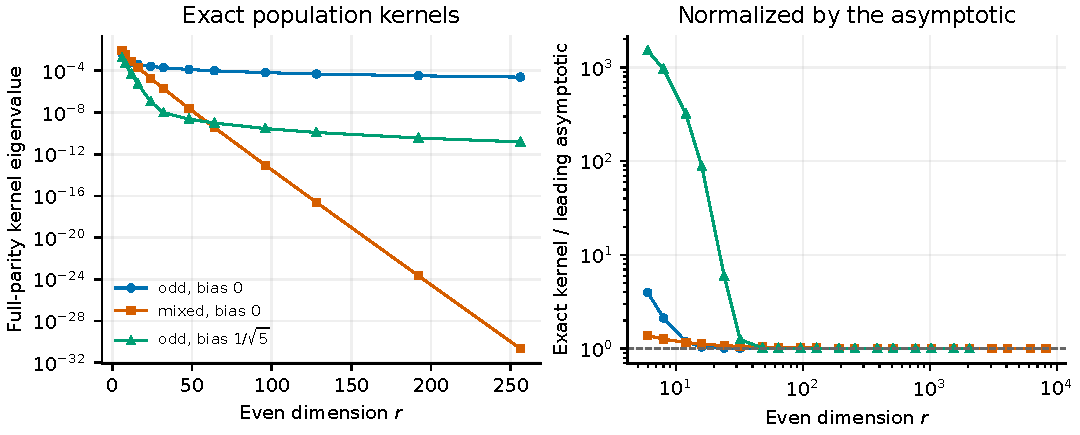
\includegraphics[width=\textwidth]{lattice-kernel-contrast.pdf}
\caption{Exact rational population calculations for the variance-one
odd and mixed four-point laws in (35)--(39). Left: zero-bias odd-lattice
features, zero-bias mixed-lattice features, and odd-lattice features at
the cancelling bias have respectively inverse-linear, exponential, and
inverse-cubic asymptotic strength. Right: the same exact values divided
by their proved leading asymptotics. Small dimensions can be far from
the asymptotic regime. Ratios involving $\pi$ use non-interval arithmetic;
the calculations support, but do not replace, the proofs.}
\end{figure}

\section*{Verification and limits}
The Fourier integral bounds, the finite-feature margin construction, and
the sequential coupling proof are conventional proofs developed and
checked in this research session. They are not independently reviewed
or Lean verified. Numerical checks accompany the integral identity and
finite-cube coefficients, but do not replace these bounds.
The threshold is a statement about polynomial versus superpolynomial
scaling, not a precise critical constant. It is stated for even full
parity and fixed even codimension, with the specified zero-bias
smoothing model; the arithmetic section separately treats hidden biases. The effect of squared-loss dynamics and of noiseless full-network
gradient descent remains open.
\end{document}
